\chapter{\IfLanguageName{dutch}{Stand van zaken}{State of the art}}%
\label{ch:stand-van-zaken}

% Tip: Begin elk hoofdstuk met een paragraaf inleiding die beschrijft hoe
% dit hoofdstuk past binnen het geheel van de bachelorproef. Geef in het
% bijzonder aan wat de link is met het vorige en volgende hoofdstuk.

% Pas na deze inleidende paragraaf komt de eerste sectiehoofding.

In this chapter the research domain of authentication is mapped out by answering a few questions that will help decide certain factors that are important for creating the fake authentication packages. Among these factors are:

\begin{itemize}
    \item the method of authenticating
    \item user role customization (+ mock data generation) %TODO weghalen
    \item security best practices
    \item creating and publishing a NuGet package
\end{itemize}

\section{State of authentication}

To discuss the factors needed to create the packages, the current state of authentication needs to be explored first.

\subsection{AAA}

When talking about authentication one often hears about triple-A. When these are mentioned they refer to: 

\begin{itemize}
    \item authentication
    \item authorization
    \item accounting
\end{itemize}

\subsubsection{Authentication}

\textcite{Magnusson2022} describes authentication as the process of identifying a user and granting them access to the network. The server evaluates the credential data submitted by the user compared to the ones stored in the network's database.

\subsubsection{Authorization}

Authorization on the other hand enforces the network policies, granular access control and user privileges. The cybersecurity AAA protocol determines which specific network resources the user has permission to access, such as a particular application, database or online service.

\subsubsection{Accounting}

Lastly, accounting is all about measuring what is happening within the network. This could mean collecting and logging data on user sessions, such as length of time, type of session, resource usage. The value here is that it offers a clear audit trail for compliance and business purposes.

\subsection{Different authentication methods}
\label{ch:different-authentication-methods}

In this day and age we have a lot more ways of authenticating a user than just writing a username or email address secured with a single password. \textcite{Maayan} lists the five most popular ways in his article and explains them.

\subsubsection{Password-based authentication}

Passwords are the most common methods of authentication. Passwords can be in the form of a string of letters, numbers, or special characters. To protect yourself you need to create strong passwords that include a combination of all possible options. 

However, passwords are prone to phishing attacks and bad hygiene that weakens effectiveness. An average person has about 25 different online accounts, but only 54\% of users use different passwords across their accounts. 

The truth is that there are a lot of passwords to remember. As a result, many people choose convenience over security. Most people use simple passwords instead of creating reliable passwords because they are easier to remember. 

The bottom line is that passwords have a lot of weaknesses and are not sufficient in protecting online information. Hackers can easily guess user credentials by running through all possible combinations until they find a match.

An article on \textcite{Descope2023} states both the pros and cons of this method. The pros being familiarity, affordability and user control, while the cons are its vulnerability, predictability, fallibility and complexity.

\subsubsection{Multi-factor authentication}

Multi-Factor Authentication (MFA) is an authentication method that requires two or more independent ways to identify a user. Examples include codes generated from the user’s smartphone, Captcha tests, fingerprints, voice biometrics or facial recognition. 

MFA authentication methods and technologies increase the confidence of users by adding multiple layers of security. MFA may be a good defence against most account hacks, but it has its own pitfalls. People may lose their phones or SIM cards and not be able to generate an authentication code.

An article on \textcite{Mitek2021} states both the benefits and costs of multi-factor authentication. The benefits are and improved user experience, greater security, protection against brute force attacks and reduced cost in the long run. The costs on the other hand are consumer friction, bias and inaccuracy, and a high implementation cost.

\subsubsection{Certificate-based authentication}

Certificate-based authentication technologies identify users, machines or devices by using digital certificates. A digital certificate is an electronic document based on the idea of a driver’s license or a passport. 

The certificate contains the digital identity of a user including a public key, and the digital signature of a certification authority. Digital certificates prove the ownership of a public key and issued only by a certification authority. 

Users provide their digital certificates when they sign in to a server. The server verifies the credibility of the digital signature and the certificate authority. The server then uses cryptography to confirm that the user has a correct private key associated with the certificate.

When looking for the advantages of certificate-based authentication, \textcite{Spector} says: `The biggest advantages of digital certificate-based authentication are privacy-based. By encrypting your communications — emails, logins or online banking transactions — digital certificates protect your private data and prevent the information from being seen by unintended eyes. Digital certificate systems are also user-friendly, usually working automatically and requiring minimal action or involvement from either senders or recipients. Microsoft states that certificate servers are cheaper and easier to manage than other certificate authorities or systems used for encryption.`

When talking about the disadvantages he says: `While the idea of digital certificates is to block outsiders from intercepting your messages, the system is not an infallible one. In 2011, for example, a Dutch digital certificate authority called DigiNotar was compromised by hackers. Since certificate authorities are the ones in charge of issuing digital certificates (think of them as the digital version of a passport office), hackers often target these authorities in order to manipulate certificate information. As a result, when a certificate authority is compromised, hackers can create websites or send emails that look genuine and pass certification tests, but are actually fraudulent.`

\subsubsection{Biometric authentication}

Biometrics authentication is a security process that relies on the unique biological characteristics of an individual. Here are key advantages of using biometric authentication technologies.

Biometric authentication technologies are used by consumers, governments and private corporations including airports, military bases, and national borders. The technology is increasingly adopted due to the ability to achieve a high level of security without creating friction for the user. Common biometric authentication methods include facial and speaker recognition and fingerprint scanners.

For the advantages \textcite{Perez2022} lists enhanced security, convenience and an improved user experience. The disadvantages that face this method are privacy concerns, false positives and again a high cost.

\subsubsection{Token-based authentication}

Token-based authentication technologies enable users to enter their credentials once and receive a unique encrypted string of random characters in exchange. You can then use the token to access protected systems instead of entering your credentials all over again. The digital token proves that you already have access permission. Use cases of token-based authentication include RESTful APIs that are used by multiple frameworks and clients.

For this implementation \textcite{Malviya} gives the major pros and cons. The pros are its scalability, efficiency, flexibility, performance and robust security. The cons are a possibility of a compromised secret key, data overhead and a shorter lifespan.

\subsection{Token-based authentication}

An article in \textcite{Okta2023}, a pioneering company in authentication that created OAuth, Okta SSO and more widely acclaimed products, lists the three different types of authentication tokens.

\begin{itemize}
    \item Connected: Keys, discs, drives, and other physical items plug into the system for access. If you've ever used a USB device or smartcard to log into a system, you've used a connected token.
    \item Contactless: A device is close enough to a server to communicate with it, but it doesn't plug in. Microsoft's so-called "magic ring" would be an example of this type of token.
    \item Disconnected: A device can communicate with the server across long distances, even if it never touches another device at all. If you've ever used your phone for a two-factor authentication process, you've used this type of token.
\end{itemize}

When thinking of the fake authentication service, it is apparent that the third option, disconnected tokens, will be the ones used in the packages.

The article also shows the four steps in the process of token authentication. First is the request. The person asks for access to a server or protected resource. That could involve a login with a password, or it could involve some other process you specify. Then comes the verification. The server determines that the person should have access. That could involve checking the password against the username, or it could involve another process you specify. After verification, the server issues a token and passes it to the user. Lastly comes storage, meaning that the token sits within the user's browser while work continues.

\subsection{Which type of method will be implemented}

When comparing the pros and cons of the methods mentioned in chapter~\ref{ch:different-authentication-methods}, token-based authentication immediately jumps out as the top candidates to implement in the fake authentication packages. With its great scalability, efficiency, flexibility and performance being very important factors for this use case. Since these packages is only meant to be used during the development stages, it is also worth mentioning that the cons are things that will not matter here. The compromised secret key can be changed during development, the shorter lifespan can be lengthened for a while and since there isn't actual data being sent to a remote server for example, the data overhead shouldn't matter that much either. All in all, this seems like the perfect candidate.

\subsection{Encoding vs Encrypting}

When certain data is transported from server to client it is often either encoded or encrypted. These are terms commonly interchanged. Both are used to transform data into a different format, but they have certain differences that are be explained by \textcite{CoderSaty}.

\subsubsection{Encrypting}

Encrypting is a process used to convert simple readable data known as plain text to unreadable data known as ciphertext which can only be converted to plain text if the user knows the encryption key. It is used basically to keep our data safe. The main purpose of the encryption is to convert our data in such a form that it is garbage for the person who does not know the encryption key. It is used to prevent unauthorized access. The reverse of encryption is decryption and it is used to get back the plain text from the ciphertext. For decryption, we must know the encryption key and the encryption algorithm \autocite{CoderSaty}. 

The encrypted data is just treated like other data. We can also use more than one encryption algorithm on the same data. The real-life examples are sending someone a secret message that only they should be able to read, or securely sending a password over the Internet. The goal is data confidentiality.

\subsubsection{Encoding}

It is the process to transform data in such a format that it can be easily used by different types of systems. The algorithm used to encode the data is publicly available and it can be easily decoded in the readable form if the person knows the algorithm. It does not require any key to decode the information. The main purpose is data usability instead of confidentiality. The main aim of encoding is to transform the data so that it can be properly used by a different type of system. It is not used to protect the data as it is easy to reverse in comparison to encryption \autocite{CoderSaty}.

Encoding is the way to go for this project since it is a developer tool, and doesn't have the need for preventing unauthorized access to the data within the token.

\subsection {Token encoding}
\label{ch:token-encoding}

Choosing an encoding method for a token involves considering various factors, like compatibility, readability, space efficiency. The most common ways used to encode a token are Uniform Resource Locator (URL), Base64, American Standard Code for Information Interchange (ASCII) and Json Web Token (JWT) encoding.

\subsubsection{URL}

URL encoding, officially known as percent-encoding, is a method to encode arbitrary data in a Uniform Resource Identifier (URI) using only the limited US-ASCII characters legal within a URI \autocite{Wikipedia2023}.

\subsubsection{Base64}

Base64 is a group of similar binary-to-text encoding schemes that represent binary data in an ASCII string format by translating it into a radix-64 representation. The term Base64 originates from a specific MIME content transfer encoding \autocite{Mozilla2023}.

When the term "Base64" is used on its own to refer to a specific algorithm, it typically refers to the version of Base64 outlined in RFC 4648, section 4, which uses the following alphabet to represent the radix-64 digits, alongside = as a padding character: ABCDEFGHIJKLMNOPQRSTUVWXYZabcdefghijklmnopqrstuvwxyz0123456789+/

\subsubsection{ASCII}

ASCII is a character encoding standard for electronic communication. ASCII codes represent text in computers, telecommunications equipment, and other devices. Because of technical limitations of computer systems at the time it was invented, ASCII has just 128 code points, of which only 95 are printable characters, which severely limited its scope. Many computer systems instead use Unicode, which has millions of code points, but the first 128 of these are the same as the ASCII set \autocite{Wikipedia2023a}.

\subsubsection{JWT}

JWT is an open standard that defines a compact and self-contained way for securely transmitting information between parties as a JSON object. This information can be verified and trusted because it is digitally signed. JWTs can be signed using a secret (with the HMAC algorithm) or a public/private key pair using RSA or ECDSA \autocite{JWT}.

In its compact form, JSON Web Tokens consist of three parts separated by dots (.), which are the header, payload and signature. Therefore, a JWT typically looks like the following: xxxxx.yyyyy.zzzzz

The header typically consists of two parts: the type of the token, which is JWT, and the signing algorithm being used, such as HMAC SHA256 or RSA. Then, this JSON is Base64Url encoded to form the first part of the JWT.

The second part of the token is the payload, which contains the claims. Claims are statements about an entity (typically, the user) and additional data. The payload is then Base64Url encoded to form the second part of the JSON Web Token.

To create the signature part you have to take the encoded header, the encoded payload, a secret, the algorithm specified in the header, and sign that.

\subsubsection{Implementing}

The goal of these packages would be to make any of these possible to implement and use, however starting out only two of these will be implemented. These packages however will be with the thought in mind that this should be as easy as possible to expand and add extra encoding methods.

As per request of Mr. Vertonghen, JWT should definitely be one of the methods implemented. Besides JWT Base64 will also be implemented, since this is one of the more basic methods of encoding binary data and it is used often in simple HTTP authentication to encode the credentials \autocite{JavaTPoint}.

\subsection{Authorization patterns}

In authorization, there are different ways a user can be given permissions. This part of the thesis goes through five of the most common ones.

\begin{itemize}
    \item Roles as User Properties
    \item Group-Based Roll-Based Access Control (RBAC)
    \item Group-Based RBAC with Fine-Grained Permissions
    \item Fine-Grained Authorization for Domain-Specific Objects
    \item Combining Group-Based RBAC and FGA
\end{itemize}

\subsubsection{Roles as User Properties}

The simplest authorization pattern models a set of roles as properties of the user. These roles can be configured in the identity provider (IDP) and are often embedded as scopes in the access token generated by the IDP \autocite{Gazitt2023}.

\subsubsection{Group-Based RBAC}

The next pattern relies on groups (and group hierarchies) as a way to organize users.

Most applications have coarse-grained roles, such as “super-admin,” “admin,”  “editor,” “viewer,” “billing-admin,” that determine permissions to objects across the entire tenant.

These roles are typically assigned by making a user a member of a group. The group membership means that the user has been granted a role. Groups can be organized into hierarchies. For example, the “auditor” group can include “internal-auditors” and “external-auditors.” These two groups can in turn include specific users \autocite{Gazitt2023}.

\subsubsection{Group-Based RBAC with Fine-Grained Permissions}

A more scalable authorization system will define a set of discrete permissions and assign those to roles. Authorization systems often define permissions as first-class concepts. Instead of checking whether a user is a member of a group, the policy can check whether a user has permission.

\subsubsection{Fine-Grained Authorization (FGA) for Domain-Specific Objects}

So far we’ve been dealing with “global” roles. Many applications want to grant permissions on a set of objects that they manage. For example, a file-sharing application such as Google Drive defines “folders” and “files” as object types. Folders and files can both have a parent folder. Each of these objects has a set of relations (“owner,” “editor,” “commenter” and “viewer”) and the “owner” can grant these roles to users and groups. So rather than a global “editor” role which has edit access to every file and folder, these permissions can be assigned to discrete folders and files.

\subsubsection{Combining Group-Based RBAC and FGA}

Most real-world applications implement some combination of group-based RBAC and fine-grained authorization. Often, authorization includes checking a global role (e.g., “editor”) and then checking whether the user has access to a particular resource (e.g., a list). The user needs to satisfy both conditions to be able to edit items on that list.

\section{NuGet package}

An essential tool for any modern development platform is a mechanism through which developers can create, share, and consume useful code. Often such code is bundled into "packages" that contain compiled code (as DLLs) along with other content needed in the projects that consume these packages. For .NET (including .NET Core), the Microsoft-supported mechanism for sharing code is NuGet, which defines how packages for .NET are created, hosted, and consumed, and provides the tools for each of those roles \autocite{Microsoft2022}.

\subsection{What is a NuGet package}

Put simply, a NuGet package is a single ZIP file with the .nupkg extension that contains compiled code (DLLs), other files related to that code, and a descriptive manifest that includes information like the package's version number. Developers with code to share create packages and publish them to a public or private host. Package consumers obtain those packages from suitable hosts, add them to their projects, and then call a package's functionality in their project code. NuGet itself then handles all of the intermediate details \autocite{Microsoft2022}.

Because NuGet supports private hosts alongside the public nuget.org host, you can use NuGet packages to share code that's exclusive to an organization or a work group. You can also use NuGet packages as a convenient way to factor your own code for use in nothing but your own projects. In short, a NuGet package is a shareable unit of code, but does not require nor imply any particular means of sharing \autocite{Microsoft2022}.

\begin{figure}
    \centering
    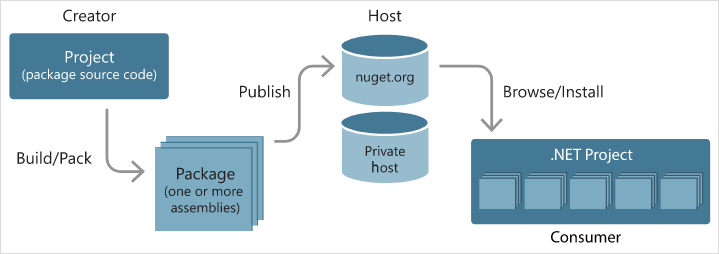
\includegraphics[scale=0.75]{nuget-flow.png}
    \caption{The flow of packages}
    \label{fig:nuget-flow}
\end{figure}

\subsection{Creating a NuGet package}

In the \textcite{Microsoft2022a} guide for package creation, it is stated that creating a package starts with the compiled code (typically .NET assemblies) that you want to package and share with others, either through the public nuget.org gallery or a private gallery within your organization. The package can also include additional files such as a readme that is displayed when the package is installed, and can include transformations to certain project files.

Creating a package is possible with the dotnet CLI, the nuget.exe CLI or MSBuild. In this case the dotnet CLI will be used.

The \textcite{Microsoft2022b} article explains all steps for creating a NuGet package using the dotnet CLI.

\subsubsection{Set properties}

You can create an example class library project by using the dotnet new classlib command, and package the project by using dotnet pack. The dotnet pack command uses the following properties.

\begin{itemize}
    \item PackageId is the package identifier and must be unique across nuget.org
    \item Version is a specific version number in the form Major.Minor.Patch[-Suffix]
    \item Authors are the authors of the package
    \item Company is company information
    \item Product is product information
\end{itemize}

If you don't specify values in the project file, the command uses default values. In Visual Studio these values can be set in the project properties.

\begin{verbatim}
    <Project Sdk="Microsoft.NET.Sdk">
        <PropertyGroup>
            <TargetFramework>netstandard2.0</TargetFramework>
            <PackageId>UniqueID</PackageId>
            <Version>1.0.0</Version>
            <Authors>Author Name</Authors>
            <Company>Company Name</Company>
            <Product>Product Name</Product>
        </PropertyGroup>
    </Project>
\end{verbatim}

The package's optional description appears on the README tab of the package's nuget.org page. The description pulls from the <Description> in the project file.

\subsubsection{Run the pack command}

To build the NuGet package or .nupkg file, run the dotnet pack command from the project folder, which also builds the project automatically. After this, the package can be published to the host of your choice.

\subsection{Publishing a NuGet package}

As stated before, NuGet packages can either be published publicly or privately. In this case, the package will be published publicly.

After creating an account on nuget.org, the next steps are needed to have a package uploaded \autocite{Microsoft2022c}:

\begin{itemize}
    \item Select Upload on the top menu at nuget.org, browse to the package on your computer, and select Open. If the package ID already exists on nuget.org, you get an error. Change the package identifier in your project, repack, and try the upload again.
    \item If the package name is available, the Verify section opens so you can review the metadata from the package manifest. If you included a readme file in your package, select Preview to make sure all content renders properly.
    \item When all the information is ready, select Submit.
\end{itemize}



